\clearpage
\addcontentsline{toc}{section}{References}
\begin{thebibliography}{99}

\addcontentsline{toc}{subsection}{\F}
\section*{\F}

\bibitem{kelly}
\begin{tabular}{p{3cm} p{7cm}}
\raisebox{-0.9\totalheight}{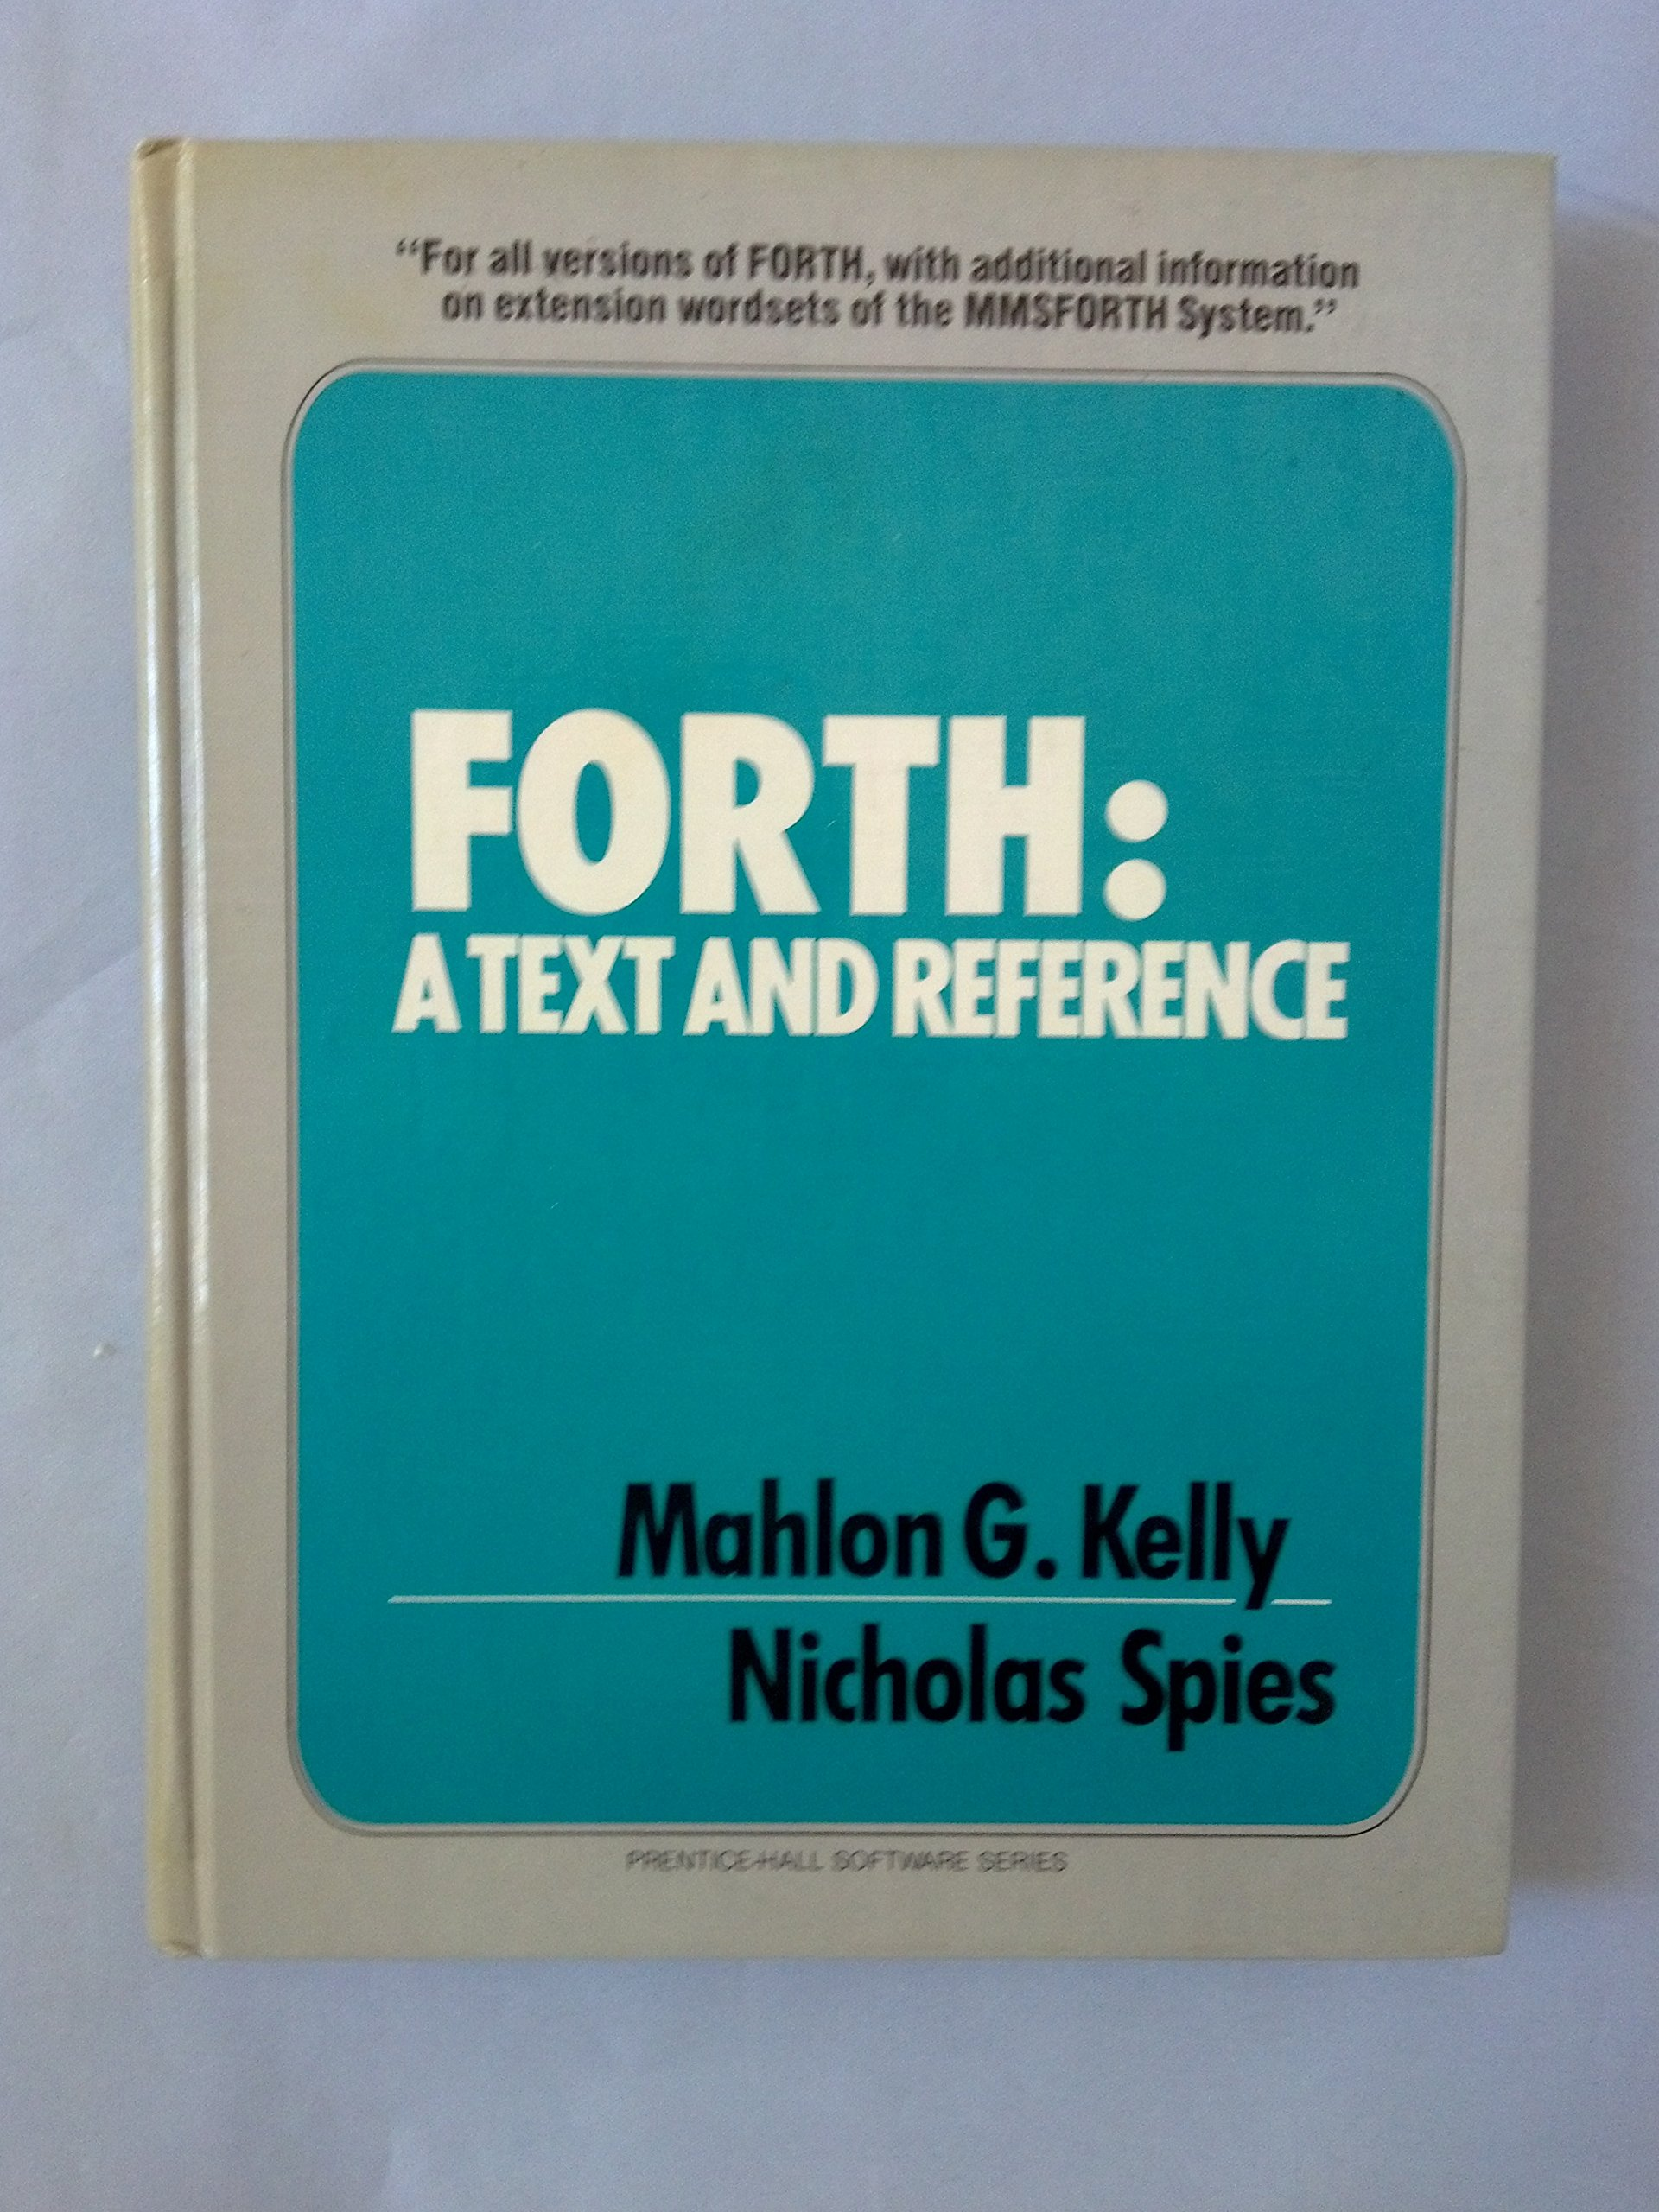
\includegraphics[width=3cm]{img/kelly_en.jpg}}&
\href{http://www.amazon.com/FORTH-Text-Reference-Prentice-Hall-software/dp/0133263495}{amazon}
\emph{\F: A Text and Reference}\par
Mahlon G. Kelly, Nicholas Spies.\\
\end{tabular}

\clearpage
\addcontentsline{toc}{subsubsection}{in russian}
\subsection*{In russian}

\bibitem{cactus} \url{http://www.forth.org.ru/~cactus/library.htm}\\
\emph{\textbf{Библиотека Доктора Кактуса}}

\bibitem{fforum} \url{http://fforum.winglion.ru/}\\
\emph{\textbf{Форум RU FIG}}

\clearpage

\bibitem{kellyru}
\begin{tabular}{p{2.5cm} p{7cm}}
\raisebox{-0.9\totalheight}{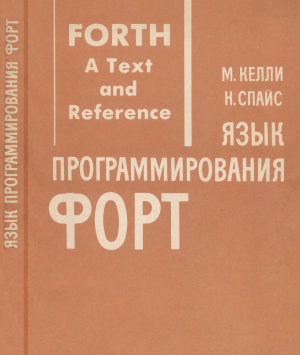
\includegraphics[width=2.5cm]{img/kelly_ru.jpg}}&
\href{http://www.forth.org.ru/~cactus/files/kelly.rar}{txt}
\emph{\textbf{Язык программирования Форт}}\par
\textbf{М.Келли, Н.Спайс}\par
{\footnotesize Перевод с английского\par Е.В. Куркова, Ю.А. Семенова.}\par
{\small Москва, <<Радио и связь>>, 1993}\\
\end{tabular}

\bibitem{baranov}
\begin{tabular}{p{2.5cm} p{7cm}}
\raisebox{-0.9\totalheight}{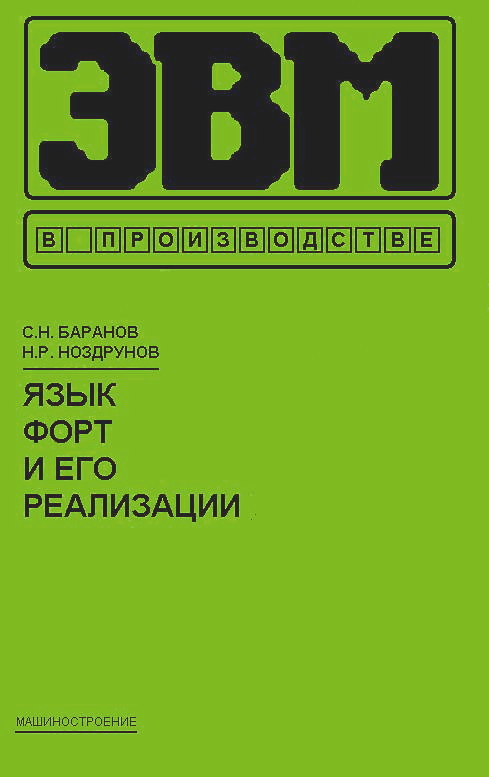
\includegraphics[width=1.9cm]{img/baranov_ru.jpg}}&
\href{http://www.forth.org.ru/~cactus/files/baranov2.rar}{txt}
\emph{\textbf{Язык Форт и его реализации}}\par
\textbf{С.Н. Баранов, Н.Р. Ноздрунов}\par
{\small Лениград, <<Машиностроение>>\par Ленинградское отделение, 1988}\\
\end{tabular}

\addcontentsline{toc}{subsection}{\ST}
\section*{\ST}

\bibitem{budd}
\begin{tabular}{p{2.5cm} p{7cm}}
\raisebox{-0.9\totalheight}{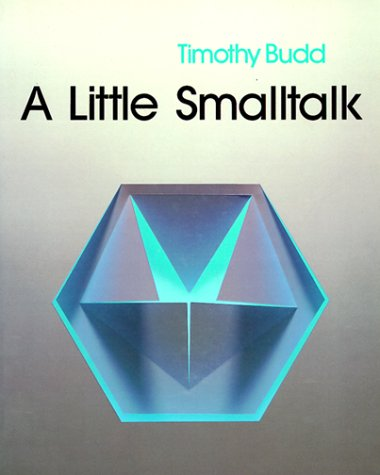
\includegraphics[width=2.5cm]{img/budd.jpg}}&
\href{http://sdmeta.gforge.inria.fr/FreeBooks/LittleSmalltalk/ALittleSmalltalk.pdf}{pdf}
\emph{\textbf{A Little Smalltalk}}\par
\textbf{Timothy Budd}\par
{\small Addison-Wesley, 1987}\\
\end{tabular}

\bibitem{STFPGA}
\href{http://esug.org/data/ESUG2014/IWST/Papers/iwst2014_From%20Smalltalk%20to%20Silicon_Towards%20a%20methodology%20to%20turn%20Smalltalk%20code%20into%20FPGA.pdf}{pdf}
\emph{\textbf{From Smalltalk to Silicon: Towards a methodology to turn Smalltalk
code into FPGA}}\\
LE Xuan Sang, Loïc Lagadec, Luc Fabresse, Jannik Laval, Noury Bouraqad

\addcontentsline{toc}{subsection}{Compilers and interpreters}
\section*{Compilers and interpreters}

\bibitem{icraft}
\url{http://www.craftinginterpreters.com/}\\
\emph{\textbf{Crafting Interpreters:\\A handbook for making programming
languages}}\\
\textbf{Bob Nystrom}

\bibitem{llvmcore}
\href{https://www.amazon.com/Getting-Started-LLVM-Core-Libraries/dp/1782166920}{Amazon}
\emph{\textbf{Getting Started with LLVM Core Libraries}}\\
\textbf{Rafael Auler}

\bibitem{dragon}
\emph{\textbf{Compilers: Principles, Techniques, and Tools}}\\
\textbf{Alfred V. Aho, Monica S. Lam, Ravi Sethi, Jeffrey D. Ullman }

\end{thebibliography}
